\documentclass[english,notes]{beamer}

% Math
\usepackage{amssymb}
\usepackage{amsmath}
\usepackage{amsfonts}
\allowdisplaybreaks{}           % Allow pagebreaks in math environments.
\makeatletter
\g@addto@macro\bfseries{\boldmath} % Typeset bold math in headings.
\makeatother

% Font
\usepackage[utf8]{inputenc}
\usepackage[T1]{fontenc}
\usepackage{babel}
\usepackage{newpxtext}
\usepackage{newpxmath}
\usepackage{microtype}

% Util package. Used for textsubscript.
\usepackage{changes}

% Captions
\usepackage[small,hang,bf,margin=30pt]{caption}

% Code listings
\usepackage{minted}
\usemintedstyle{bw}

% Colors
\usepackage{color}
\definecolor{my-red}{HTML}{E41A1C}
\definecolor{my-green}{HTML}{4DAF4A}
\definecolor{my-blue}{HTML}{377EB8}
\definecolor{my-purple}{HTML}{984EA3}
\definecolor{my-orange}{HTML}{FF7F00}

% Graphics
\usepackage{graphicx}
\usepackage{subcaption}
\usepackage{float}
\usepackage{tikz}
\usepackage{pgfplots}
\usetikzlibrary{patterns}
% \usetikzlibrary{external}
% \tikzexternalize[prefix=tikz/,mode=list and make]
% \pgfkeys{/pgf/images/include external/.code=\includegraphics{#1}} % Makes
                                                                  % externalize
                                                                  % and draft
                                                                  % work
                                                                  % together.
\pgfplotsset{%
  % invoke before crossref tikzpicture={\tikzexternaldisable},
  % invoke after crossref tikzpicture={\tikzexternalenable},
  ylabel near ticks,
  legend columns=-1,
  legend style={at={(0.5, 1)},anchor=south,draw=none,fill=none,/tikz/every even
    column/.append style={column sep=10pt}},
  every y tick scale label/.style={at={(0,1)},anchor=east, font=\scriptsize,
    inner xsep=2pt, inner ysep=0pt},
  ytick placement tolerance=-2mm,
  max space between ticks=30pt,
}
\usetikzlibrary{arrows}
\usepgfplotslibrary{groupplots}

\tikzset{%
    viterbi-l/.style={%
      only marks, mark=*, color=my-red
    },
    viterbi-p/.style={%
      only marks, mark=square*, color=my-green
    },
    viterbi-pm/.style={%
      only marks, mark=triangle*, color=my-blue
    },
    indexed-one/.style={%
      only marks, mark=*, color=my-red
    },
    indexed-many/.style={%
      only marks, mark=square*, color=my-green
    },
}


% Fixme
\usepackage[draft]{fixme}
\fxsetup{inlineface=\bfseries\tiny,inline=true,nomargin}

% Colors
\usepackage{color}
\definecolor{my-red}{HTML}{E41A1C}
\definecolor{my-green}{HTML}{4DAF4A}
\definecolor{my-blue}{HTML}{377EB8}
\definecolor{my-purple}{HTML}{984EA3}
\definecolor{my-orange}{HTML}{FF7F00}

% User defined macros
\DeclareMathOperator*{\argmin}{arg\,min}
\DeclareMathOperator*{\argmax}{arg\,max}

% Date
\usepackage{datetime}

% Beamer stuff.
\usetheme{default}
\setbeamertemplate{navigation symbols}{}
\AtBeginSection[]
{
 \begin{frame}<beamer>
 \frametitle{Agenda}
 \tableofcontents[currentsection]
 \end{frame}
}
\usefonttheme{serif}

% Symbols
\usepackage[weather]{ifsym}
\newcommand{\sun}{\text{\Sun}}
\newcommand{\cloud}{\text{\Cloud}}
\newcommand{\rain}{\text{\Rain}}
\newcommand{\suncloud}{\text{\SunCloud}}

\title{Speeding Up HMM Decoding Using Compression}
\author{Torben Muldvang Andersen, 20093713}
\date{\protect\formatdate{24}{06}{2015}}

\begin{document}
\begin{frame}
  \maketitle
  
\includegraphics[height=7mm, trim=0 0 40mm 0, clip]{../logo}
  \hfill
  
\includegraphics[height=7mm]{../BiRC-logo}
\end{frame}

\begin{frame}
  \frametitle{Agenda}
    Med udgangspunkt i specialerapporten ønskes et foredrag, hvor de
    væsentligste resultater af specialeprojektet fremlægges.
  \begin{itemize}
  \item Du bedes presentere hvorledes skjulte Markov modeller anvendes til
    Viterbi- og Posterior-decoding med fokus på hvorledes implementeringen af
    disse decoding-methoder kan formuleres ved hjælp af lineær algebra samt
    hvorledes en præprocessesing med henblik på en ``komprimering'' af input
    kan forbedre deres kørselstid i praksis.
  \item Du bedes også præsentere dine implementeringer af metoderne og
    udvidelser til biblioteket zipHMMlib samt de eksperimenter som du har
    gennemført for at undersøge deres kørselstider i praksis, herunder hvornår
    præprocesseringen giver den ønskede forbedring af kørselstiden.
  \item Endelig bedes du overveje hvorvidt andre former for præprocessering
    (komprimering) kunne anvedes.
  \end{itemize}
\end{frame}

\begin{frame}
  \frametitle{Agenda}
  \tableofcontents{}
\end{frame}

\section{Goal}

\begin{frame}
  \frametitle{\insertsection}
  Complement the work made by Sand et al. (2013).
  \begin{itemize}
  \item Decoding algorithms: Viterbi and posterior decoding.
  \item Theory, implementation, experiments.
  \end{itemize}
\end{frame}

\section{Hidden Markov Models}

\begin{frame}
  \frametitle{\insertsection}
  \begin{columns}
    \onslide<+->
      \begin{column}{0.5\textwidth}
        \centering
        \tikzsetnextfilename{HMM}
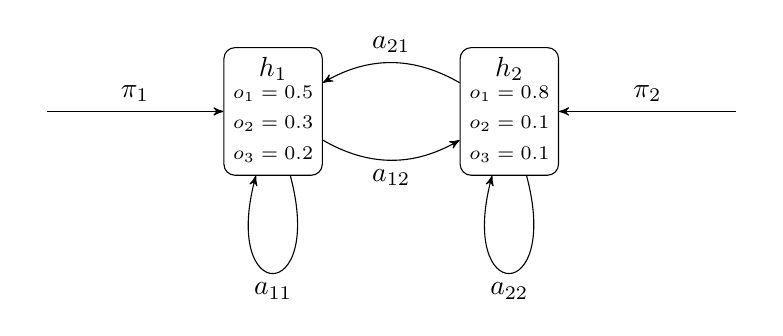
\begin{tikzpicture} [
  ->,
  >=stealth',
  auto,
  node distance=3cm,
  main node/.style={rectangle,draw,rounded corners,align=center},
  ]

  \node[main node] (h1) {$h_1$\\{\scriptsize%
    $\begin{aligned}
        o_1 &= 0.5\\ o_2 &= 0.3\\ o_3 &= 0.2\\
    \end{aligned}$}};
  \node[main node, right of=h1] (h2) {$h_2$\\{\scriptsize%
    $\begin{aligned}
        o_1 &= 0.8\\ o_2 &= 0.1\\ o_3 &= 0.1\\
    \end{aligned}$}};
  \node[left of=h1] (p1) {};
  \node[right of=h2] (p2) {};

  \path
    (h1) edge[bend right]               node[below] {$a_{12}$} (h2)
         edge[loop below, looseness=10] node        {$a_{11}$} (h1)
    (h2) edge[bend right]               node[above] {$a_{21}$} (h1)
         edge[loop below, looseness=10] node        {$a_{22}$} (h2);

  \path
    (p1) edge node[above] {$\pi_1$} (h1)
    (p2) edge node[above] {$\pi_2$} (h2);
\end{tikzpicture}

%%% Local Variables:
%%% mode: latex
%%% TeX-master: "../master"
%%% End:

      \end{column}%
    \onslide<+->{
      \begin{column}{0.5\textwidth}
        \begin{tabular}{rl}
          Hidden states                 & L H                                                                                    \\
          Observables                   & \Sun{} \Cloud{} \Rain{}                                                                \\
        \end{tabular}
      \end{column}}
  \end{columns}
  \onslide<+->{
    \begin{center}
      \begin{tabular}{rcccccccccc}
        Observation $Y_{1:T}$           & \Sun{} & \Sun{} & \Cloud{} & \Rain{} & \Sun{} & \Cloud{} & \Sun{} & \Cloud{} & \Rain{} \\
        \onslide<+-> Decoding $X_{1:T}$ & H      & H      & H        & L       & L      & H        & H      & H        & H       \\
      \end{tabular}
    \end{center}}
\end{frame}

\section{Viterbi Decoding}

\subsection{The Original Viterbi Algorithm}
\begin{frame}
  \frametitle{\insertsubsection}
  \onslide<+->
  Given a model $\lambda$ and an observation sequence $Y_{1:T}$, define
  \begin{equation*}
    \delta_t(x_t) = \max_{x_{1:t}} \Pr(Y_{1:t}, X_{1:t} = x_{1:t} \mid \lambda).
  \end{equation*}

  \onslide<+->
  This can be solved by dynamic programming using
  \begin{equation*}
    \begin{aligned}
      \delta_1(x_1) &= \pi_{x_1} b_{x_1, y_1} \\
      \delta_t(x_t) &= \max_{x_{t - 1}} \delta_{t - 1}(x_{t - 1}) a_{x_{t - 1}, x_t} b_{x_t, y_t} .
    \end{aligned}
  \end{equation*}

  \onslide<+->
  \begin{center}
    %\tikzsetnextfilename{viterbi}
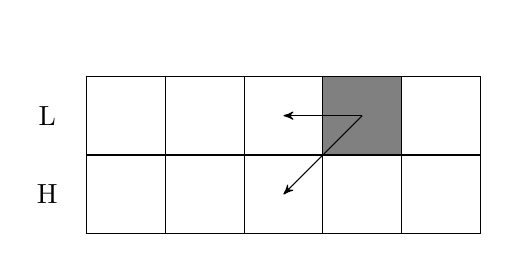
\begin{tikzpicture} [
  ->,
  >=stealth',
  ]
  \tikzstyle{box} = [draw=black, minimum width=10mm, minimum height=10mm];

  \node at (0, 1) {H};
  \node at (0, 2) {L};

  \node[box] at (1, 1) {};
  \node[box] at (1, 2) {};
  \node[box] at (2, 1) {};
  \node[box] at (2, 2) {};
  \node[box] at (3, 1) {};
  \node[box] at (3, 2) {};
  \node[box] at (4, 1) {};
  \node[box] at (4, 2) {};
  \node[box] at (5, 1) {};
  \node[box] at (5, 2) {};

  \node at (1, 3) {\Sun};
  \node at (2, 3) {\Sun};
  \node at (3, 3) {\Cloud};
  \node at (4, 3) {\Sun};
  \node at (5, 3) {\Sun};

  \onslide<+->
  \node[box,fill=gray] at (4, 2) {};
  \draw (4, 2) -- (3, 2);
  \draw (4, 2) -- (3, 1);
\end{tikzpicture}

%%% Local Variables:
%%% mode: latex
%%% TeX-master: "../master"
%%% End:

  \end{center}

  \onslide<6->{
    Backtracking using argmax table to obtain $V_{1:T}$.
  }

  \onslide<8->{
    Running time: $O(N^2 T)$
  }

 \fxwarning{Forklar øverste notation.}
 \fxwarning{Forbered udledning af Viterbi.}
\end{frame}

\subsection{Linear Algebra}

\begin{frame}
  \frametitle{\insertsubsection}
  \onslide<+->{
    \begin{equation*}
      \Pi =
      \begin{bmatrix}
        \pi_1                            \\
        \vdots                           \\
        \pi_N                            \\
      \end{bmatrix}\quad
      A =
      \begin{bmatrix}
        a_{1, 1}   & \cdots & a_{1,N}    \\
        \vdots     & \ddots & \vdots     \\
        a_{N, 1}   & \cdots & a_{N,N}    \\
      \end{bmatrix}\quad
      B_{o_i} =
      \begin{bmatrix}
        b_{1, o_i} &        &            \\
        & \ddots &            \\
        &        & b_{N, o_i} \\
      \end{bmatrix}
    \end{equation*}
  }

  \onslide<+->{
    \begin{equation*}
      \delta_t(x_t) = \max_{x_{t - 1}} \delta_{t - 1}(x_{t - 1}) \underbrace{a_{x_{t - 1},x_t} b_{x_t, y_t}}_{\textstyle C_{o_i} = B_{o_i} A^T}
    \end{equation*}
  }

  \onslide<+->{
    \begin{equation*}
      \begin{aligned}
        \delta_1 &= C_1 = B_{y_1} \Pi\\
        \onslide<+-> \delta_t &= C_{y_t} \odot \delta_{t - 1} = C_{y_t} \odot C_{y_{t-1}} \odot \dots \odot C_1
      \end{aligned}
    \end{equation*}
  }

  \onslide<+->
  Running time: $O(M N^3 + N^2 T)$

  \vfill
  \fxwarning{Reformulation. (Would be really cool if this could be made using an
    illustration of the stuff multiplied in the original algorithm and the
    table using the weather example.)}
  \fxwarning{In the implementation the matrixmultiplications involving
    $B_{o_i}$ takes time $O(N^2)$ since $B$ is stored as an array.}
\end{frame}

\subsection{Exploiting Repetitions}

\begin{frame}
  \frametitle{\insertsubsection}
  Example
  \begin{center}
    \def\tabcolsep{1pt}
    \begin{tabular}{rccccccccccccccccc}
      \onslide<1->{$\delta_{T} =$ & $C_{\rain}$ & $\odot$ & \alert<2->{$C_{\cloud}$} & \alert<2->{$\odot$} & \alert<2->{$C_{\sun}$} & $\odot$ & \alert<2->{$C_{\cloud}$} & \alert<2->{$\odot$} & \alert<2->{$C_{\sun}$} & $\odot$ & $C_{\rain}$ & $\odot$ & \alert<2->{$C_{\cloud}$} & \alert<2->{$\odot$} & \alert<2->{$C_{\sun}$} & $\odot$ & $C_1$ \\}%
      \onslide<3->{$ =$  & $C_{\rain}$ & $\odot$ & \multicolumn{3}{c}{$C_{\suncloud}$} & $\odot$ & \multicolumn{3}{c}{$C_{\suncloud}$} & $\odot$ & $C_{\rain}$ & $\odot$ & \multicolumn{3}{c}{$C_{\suncloud}$} & $\odot$ & $C_1$ \\}%
    \end{tabular}
  \end{center}
  \onslide<4->{
    Byte-pair encoding
  }
  \begin{center}
    \def\tabcolsep{1pt}
    \begin{tabular}{ccccccccccccccccc}
    \onslide<5->{$Y_{1:T} = $ & \Sun{} & \alert<6->{\Sun{}} & \alert<6->{\Cloud{}} & \Rain{} & \alert<6->{\Sun{}} & \alert<6->{\Cloud{}} & \alert<6->{\Sun{}} & \alert<6->{\Cloud{}} & \Rain{} \\}%
    \onslide<7->{& \Sun{} & \multicolumn{2}{c}{\alert<8->{\SunCloud{}}} & \alert<8->{\Rain{}} & \multicolumn{2}{c}{\SunCloud{}} & \multicolumn{2}{c}{\alert<8->{\SunCloud{}}} & \alert<8->{\Rain{}} \\}%
    \onslide<9-> $Y_{1:T'}' = $ & \Sun{} & & \Lightning{} & & \multicolumn{2}{c}{\SunCloud{}} & & \Lightning{} & \\
    \end{tabular}
  \end{center}
\end{frame}

\begin{frame}
  \frametitle{Backtracking}
  \onslide<1->{
    From argmax table $V_{1:T'}'$ can be obtained.
    \begin{center}
      \begin{tikzpicture} [
  ->,
  >=stealth',
  ]
  \tikzstyle{box} = [draw=black, minimum width=10mm, minimum height=10mm];

  \node at (0, 1) {H};
  \node at (0, 2) {L};

  \node at (1, 0) {\Sun};
  \node at (4, 0) {\Lightning};
  \node at (6, 0) {\SunCloud};
  \node at (9, 0) {\Lightning};

  \node[box, fill=gray] at (1, 1) {};
  \node[box, fill=gray] at (1, 2) {};
  \node[box] at (2, 1) {};
  \node[box] at (2, 2) {};
  \node[box] at (3, 1) {};
  \node[box] at (3, 2) {};
  \node[box, fill=gray] at (4, 1) {};
  \node[box, fill=gray] at (4, 2) {};
  \node[box] at (5, 1) {};
  \node[box] at (5, 2) {};
  \node[box, fill=gray] at (6, 1) {};
  \node[box, fill=gray] at (6, 2) {};
  \node[box] at (7, 1) {};
  \node[box] at (7, 2) {};
  \node[box] at (8, 1) {};
  \node[box] at (8, 2) {};
  \node[box, fill=gray] at (9, 1) {};
  \node[box, fill=gray] at (9, 2) {};

  \node at (1, 3) {\Sun};
  \node at (2, 3) {\Sun};
  \node at (3, 3) {\Cloud};
  \node at (4, 3) {\Rain};
  \node at (5, 3) {\Sun};
  \node at (6, 3) {\Cloud};
  \node at (7, 3) {\Sun};
  \node at (8, 3) {\Cloud};
  \node at (9, 3) {\Rain};

  \draw (9, 2) -- (6, 1);
  \draw (4, 2) -- (1, 1);

  \onslide<1-2>{
    \draw (6, 1) -- (4, 2);
  }

  \onslide<3->{
    \draw<3-> (6, 1) -- (5, 1);
    \draw<3-> (5, 1) -- (4, 2);
  }
\end{tikzpicture}

%%% Local Variables:
%%% mode: latex
%%% TeX-master: "../master"
%%% End:

    \end{center}
  }

  \onslide<2->{
    Compute another set of matrices.
    \begin{equation*}
      C_{\suncloud} = C_{\cloud} \odot C_{\sun}, \quad
      R_{\suncloud}(i, j) = \argmax_k
      \left(
        C_{\cloud}(i, k) \cdot C_{\sun}(k, j)
      \right).
    \end{equation*}
  }

  \onslide<4->{
    Running time: $O(M' N^3 + N^2 T')$ or $O(M' N^3 + N^2 T' + T)$.
  }
\end{frame}
\section{Posterior Decoding}

\begin{frame}
  \frametitle{\insertsection}
  \onslide<+->
  Given a model $\lambda$ and an observation sequence $Y_{1:T}$,
  find the most likely state at the time the symbol is emitted.
  \begin{equation*}
    \begin{aligned}
      p_t & = \argmax_{x_t \in \mathcal{H}} \Pr \left(x_t | Y_{1:T}, \lambda \right) \\
          \onslide<+-> & = \argmax_{x_t \in \mathcal{H}} \alpha(x_t) \beta(x_t).
    \end{aligned}
  \end{equation*}
  \onslide<+->
  Problems in exploiting repetitions:
  \begin{itemize}
  \item<+-> No dependence between sequential states in posterior decoding.
  \item<+-> Computation of full tables cannot be sped up.
  \end{itemize}
\end{frame}

\section{Indexed Posterior Decoding}

\begin{frame}
  \frametitle{\insertsection}
  \onslide<+->
  Given a model $\lambda$ and an observation sequence $Y_{1:T}$, find the
  posterior decoding $P_{i:j}$.

  \begin{overlayarea}{\textwidth}{3cm}
    \only<+>{
      \begin{center}
        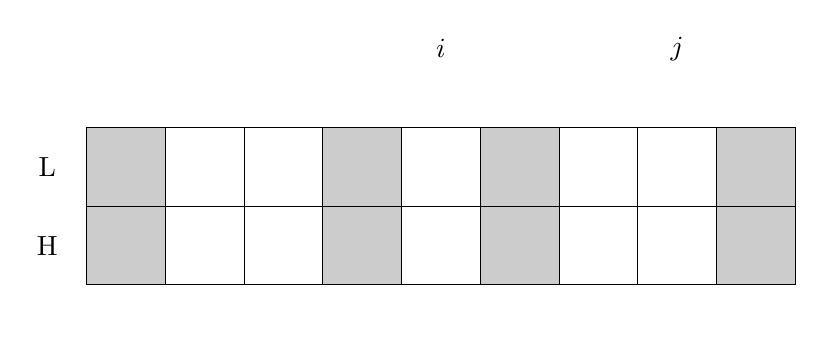
\begin{tikzpicture} [
  ->,
  >=stealth',
  ]
  \tikzstyle{box} = [draw=black, minimum width=10mm, minimum height=10mm];

  \node at (0, 1) {H};
  \node at (0, 2) {L};

  \node at (1, 0) {\Sun};
  \node at (4, 0) {\Lightning};
  \node at (6, 0) {\SunCloud};
  \node at (9, 0) {\Lightning};

  \node[box, fill=black!20!white] at (1, 1) {};
  \node[box, fill=black!20!white] at (1, 2) {};
  \node[box] at (2, 1) {};
  \node[box] at (2, 2) {};
  \node[box] at (3, 1) {};
  \node[box] at (3, 2) {};
  \node[box, fill=black!20!white] at (4, 1) {};
  \node[box, fill=black!20!white] at (4, 2) {};
  \node[box] at (5, 1) {};
  \node[box] at (5, 2) {};
  \node[box, fill=black!20!white] at (6, 1) {};
  \node[box, fill=black!20!white] at (6, 2) {};
  \node[box] at (7, 1) {};
  \node[box] at (7, 2) {};
  \node[box] at (8, 1) {};
  \node[box] at (8, 2) {};
  \node[box, fill=black!20!white] at (9, 1) {};
  \node[box, fill=black!20!white] at (9, 2) {};

  \node at (1, 3) {\Sun};
  \node at (2, 3) {\Sun};
  \node at (3, 3) {\Cloud};
  \node at (4, 3) {\Rain};
  \node at (5, 3) {\Sun};
  \node at (6, 3) {\Cloud};
  \node at (7, 3) {\Sun};
  \node at (8, 3) {\Cloud};
  \node at (9, 3) {\Rain};

  \node at (5, 3.5) {$i$};
  \node at (8, 3.5) {$j$};
\end{tikzpicture}

%%% Local Variables:
%%% mode: latex
%%% TeX-master: "../master"
%%% End:

      \end{center}
    }

    \only<+->{
      \begin{center}
        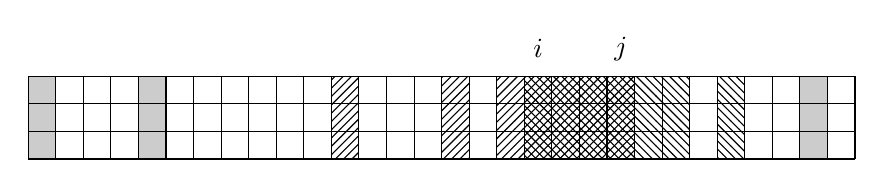
\begin{tikzpicture} [
  scale=0.35,
  ]

  \node at (18.5, 4) {$i$};
  \node at (21.5, 4) {$j$};

  \fill[black!20!white] (0, 0) rectangle (1,3);
  \fill[black!20!white] (4, 0) rectangle (5,3);
  \fill[black!20!white] (28, 0) rectangle (29,3);

  \draw (0, 0) grid (30, 3);

  \only<+->{
    \draw[pattern=north east lines] (11, 0) rectangle (12, 3);
    \draw[pattern=north east lines] (15, 0) rectangle (16, 3);
    \draw[pattern=north east lines] (17, 0) rectangle (18, 3);

    \draw[pattern=north east lines] (18, 0) rectangle (19, 3);
    \draw[pattern=north east lines] (19, 0) rectangle (20, 3);
    \draw[pattern=north east lines] (20, 0) rectangle (21, 3);
    \draw[pattern=north east lines] (21, 0) rectangle (22, 3);
  }

  \only<+->{
    \draw[pattern=north west lines] (25, 0) rectangle (26, 3);
    \draw[pattern=north west lines] (23, 0) rectangle (24, 3);
    \draw[pattern=north west lines] (22, 0) rectangle (23, 3);

    \draw[pattern=north west lines] (18, 0) rectangle (19, 3);
    \draw[pattern=north west lines] (19, 0) rectangle (20, 3);
    \draw[pattern=north west lines] (20, 0) rectangle (21, 3);
    \draw[pattern=north west lines] (21, 0) rectangle (22, 3);
  }

\end{tikzpicture}

%%% Local Variables:
%%% mode: latex
%%% TeX-master: "../master"
%%% End:

      \end{center}
    }
  \end{overlayarea}

  \onslide<+-> {
    Running time: $O(M' N^3 + N^2 T' + N^2 (j - i + \log T))$.
  }
\end{frame}

\section{Implementation}

\begin{frame}[fragile]
  \frametitle{\insertsection}
\begin{minted}[fontsize=\tiny]{C++}
void HMMSuite::read_seq(std::string &seq_filename, size_t alphabet_size,
                        size_t no_states, size_t min_no_eval)

double HMMSuite::forward(Matrix &pi, Matrix &A, Matrix &B)

double HMMSuite::forward(Matrix &pi, Matrix &A, Matrix &B,
                         std::vector<double> &scales,
                         Matrix *forward_table)

void HMMSuite::backward(Matrix &pi, Matrix &A, Matrix &B,
                        std::vector<double> &scales,
                        Matrix *backward_table)

double HMMSuite::viterbi(Matrix &pi, Matrix &A, Matrix &B,
                         bool memory_save,
                         std::vector<unsigned> &viterbi_path)

void HMMSuite::posterior_decoding(Matrix &pi,  Matrix &A,  Matrix &B,
                                  std::vector<unsigned> &posterior_path)

void HMMSuite::indexed_posterior_decoding(Matrix &pi,  Matrix &A,  Matrix &B,
                                          size_t i, size_t j,
                                          std::vector<unsigned> &posterior_path)
\end{minted}
\end{frame}

\section{Experiments}

\begin{frame}
  \frametitle{\insertsection}
  Setup etc.
  \begin{itemize}
    \tiny
  \item Main experiments.
  \item Some kind of summary of experiments
  \end{itemize}
\end{frame}

\begin{frame}
  \frametitle{Before}
\begin{figure}
  \centering\ref{legend:before_simple_random_vs_fib}
  \begin{subfigure}{0.5\textwidth}
    \centering
    \begin{tikzpicture}[trim axis left,trim axis right]
      \begin{axis}[
        xlabel=Sequence length $T$,
        ylabel=$\frac{\text{Running time}}{T}$,
        width=\textwidth,
        height=0.9\textwidth,
        xmode=log,
        ymax=0.000025,
        ymin=-0.000001,
        legend entries={Original Viterbi\textsubscript{P}, Original Viterbi\textsubscript{L}},
        legend to name=legend:before_simple_random_vs_fib,
        ]
        \addplot[viterbi-p, error bars, y dir=both, y explicit]
        table[x=T, y=simple_path_total_time/T, y error=simple_path_total_time/T_std]
        {../plot_data/viterbi_sequence_transformed.data};

        \addplot[viterbi-l, error bars, y dir=both, y explicit]
        table[x=T, y=simple_total_time/T, y error=simple_total_time/T_std]
        {../plot_data/viterbi_sequence_old_transformed.data};
      \end{axis}
    \end{tikzpicture}
    \caption{Random sequences.}
  \end{subfigure}%
  \begin{subfigure}{0.5\textwidth}
    \centering
    \begin{tikzpicture}[trim axis left,trim axis right]
      \begin{axis}[
        xlabel=Sequence length $T$,
        width=\textwidth,
        height=0.9\textwidth,
        xmode=log,
        ymax=0.000025,
        ymin=-0.000001,
        ]
        \addplot[viterbi-p, error bars, y dir=both, y explicit]
        table[x=T, y=simple_path_total_time/T, y error=simple_path_total_time/T_std]
        {../plot_data/viterbi_fib_sequence_transformed.data};

        \addplot[viterbi-l, error bars, y dir=both, y explicit]
        table[x=T, y=simple_total_time/T, y error=simple_total_time/T_std]
        {../plot_data/viterbi_fib_sequence_transformed.data};
      \end{axis}
    \end{tikzpicture}
    \caption{Fibonacci words.}
  \end{subfigure}
\end{figure}
\end{frame}

\begin{frame}
  \frametitle{After}
\begin{figure}
  \centering\ref{legend:simple_random_vs_fib}
  \begin{subfigure}{0.5\textwidth}
    \centering
    \begin{tikzpicture}[trim axis left,trim axis right]
      \begin{axis}[
        xlabel=Sequence length $T$,
        ylabel=$\frac{\text{Running time}}{T}$,
        width=\textwidth,
        height=0.9\textwidth,
        xmode=log,
        ymax=0.000002,
        ymin=0,
        legend entries={Original Viterbi\textsubscript{P}, Original Viterbi\textsubscript{L}},
        legend to name=legend:simple_random_vs_fib,
        ]
        \addplot[viterbi-p, error bars, y dir=both, y explicit]
        table[x=T, y=simple_path_total_time/T, y error=simple_path_total_time/T_std]
        {../plot_data/viterbi_sequence_transformed.data};

        \addplot[viterbi-l, error bars, y dir=both, y explicit]
        table[x=T, y=simple_total_time/T, y error=simple_total_time/T_std]
        {../plot_data/viterbi_sequence_transformed.data};
      \end{axis}
    \end{tikzpicture}
    \caption{Random sequences.}
  \end{subfigure}%
  \begin{subfigure}{0.5\textwidth}
    \centering
    \begin{tikzpicture}[trim axis left,trim axis right]
      \begin{axis}[
        xlabel=Sequence length $T$,
        width=\textwidth,
        height=0.9\textwidth,
        xmode=log,
        ymax=0.000002,
        ymin=0,
        ]
        \addplot[viterbi-p, error bars, y dir=both, y explicit]
        table[x=T, y=simple_path_total_time/T, y error=simple_path_total_time/T_std]
        {../plot_data/viterbi_fib_sequence_transformed.data};

        \addplot[viterbi-l, error bars, y dir=both, y explicit]
        table[x=T, y=simple_total_time/T, y error=simple_total_time/T_std]
        {../plot_data/viterbi_fib_sequence_transformed.data};
      \end{axis}
    \end{tikzpicture}
    \caption{Fibonacci words.}
  \end{subfigure}
\end{figure}
\end{frame}

\section{Other Types of Preprocessing}

\begin{frame}
  \frametitle{\insertsection}

\end{frame}
\end{document}



%%% Local Variables:
%%% mode: latex
%%% TeX-command-extra-options: "-shell-escape"
%%% TeX-master: t
%%% End:
